\documentclass[letterpaper,11pt]{article}
\oddsidemargin -1.0cm \textwidth 17.5cm

\usepackage[utf8]{inputenc}
\usepackage[activeacute,spanish, es-lcroman]{babel}
\decimalpoint
\usepackage{amsfonts,setspace}
\usepackage{amsmath}
\usepackage{amssymb, amsmath, amsthm}
\usepackage{comment}
\usepackage{float}
\usepackage{amssymb}
\usepackage{dsfont}
\usepackage{anysize}
\usepackage{multicol}
\usepackage{enumerate}
\usepackage{graphicx}
\usepackage[left=1.5cm,top=2cm,right=1.5cm, bottom=1.7cm]{geometry}
\setlength\headheight{1.5em} 
\usepackage{fancyhdr}
\usepackage{multicol}
\usepackage{hyperref}
\usepackage{wrapfig}
\usepackage{subcaption}
\usepackage{siunitx}
\usepackage{cancel}
\usepackage{mdwlist}
\usepackage{svg}
\pagestyle{fancy}
\fancyhf{}
\renewcommand{\labelenumi}{\normalsize\bfseries P\arabic{enumi}.}
\renewcommand{\labelenumii}{\normalsize\bfseries (\alph{enumii})}
\renewcommand{\labelenumiii}{\normalsize\bfseries \roman{enumiii})}


\begin{document}

\fancyhead[L]{\itshape{Facultad de Ciencias F\'isicas y Matem\'aticas}}
\fancyhead[R]{\itshape{Universidad de Chile}}

\begin{minipage}{11.5cm}
    \begin{flushleft}
        \hspace*{-0.6cm}\textbf{FI1000-1 Introducción a la Física Clásica}\\
        \hspace*{-0.6cm}\textbf{Profesor:} Ignacio Bordeu\\
        \hspace*{-0.6cm}\textbf{Auxiliares:} Alejandro Cartes \& Simón Yáñez\\
        \hspace*{-0.6cm}\textbf{Ayudante:} Javier Cubillos\\
    \end{flushleft}
\end{minipage}

\begin{picture}(2,3)
    \put(366, 10){
\includegraphics[scale=0.9]{2020-1/Imágenes/logo/dfi-fcfm.pdf}}
\end{picture}

\begin{center}
	\LARGE\textbf{Trabajo Dirigido \#2}\\
	\Large{Preparación C1}
\end{center}

\vspace{-1cm}
\begin{enumerate}\setlength{\itemsep}{0.4cm}

\rfoot[]{pág. \thepage}

\item[]

% ---------------------------------------------------------
% ando sin inspiración :( no encontré más ejercicios buenos
% ---------------------------------------------------------

\item Un viernes por la mañana, un papá quiere ir a dejar a su pequeño hijo al colegio. El papá se sube al auto y comienza a conducir con una rapidez constante $v_a$. Tras haber recorrido una distancia $L$ se percata que su hijo nunca se subió al auto, por lo que decide frenar con aceleración $a_{0}$ y retroceder hacia el punto de partida bajo la misma aceleración. Cuando vuelve a pasar por la distancia $L$, el padre acelera el automóvil de tal manera que pueda llegar con una velocidad nula hasta donde se encuentra su hijo, permitiéndole subir al auto.

\begin{enumerate}
    \item Determine la aceleración del último trayecto
    \item Determine cuánto tiempo estuvo el niño esperando
\end{enumerate}

\item Una pelota es lanzada desde la base de una colina con un ángulo de lanzamiento $\alpha$ con respecto a la horizontal y una velocidad inicial $v_0$. Si La colina tiene un ángulo de elevación $\delta$, determine la distancia horizontal que la pelota recorre a lo largo de la colina.
    
\begin{figure}[H]
    \centering
    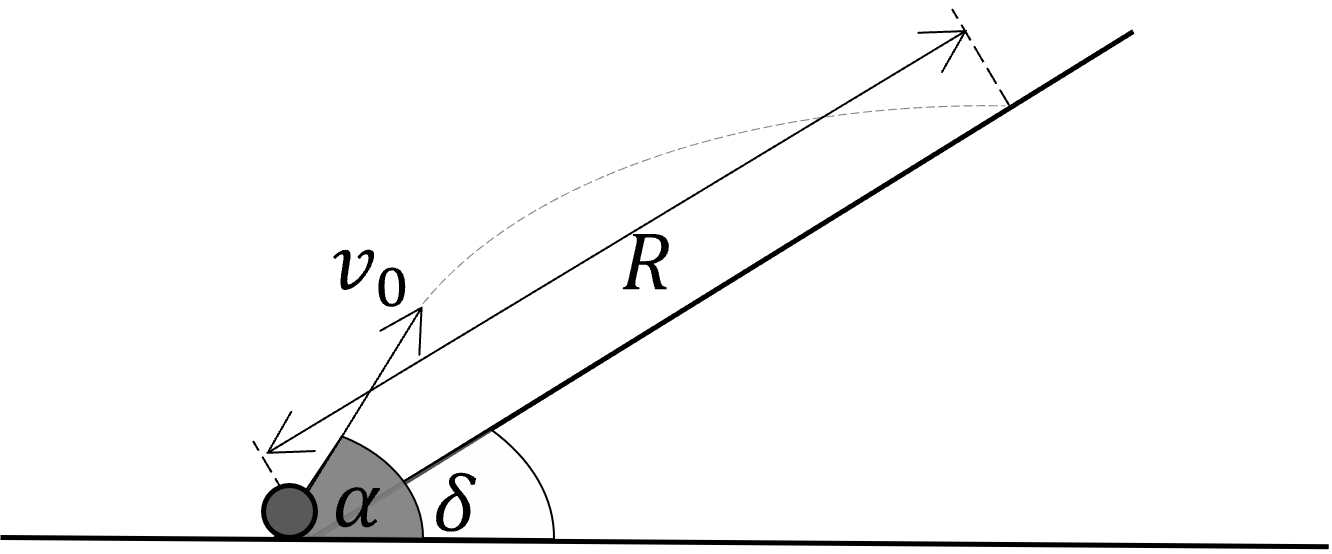
\includegraphics[width=0.4\linewidth]{2023-1/img/TD 2/plano.png}
\end{figure}


\item 
\begin{enumerate}
    \item Una piedra atada a una cuerda de largo $L$ se hace rotar de manera vertical. En cierto instante, la cuerda se corta como se muestra en la figura. Si la altura máxima alcanzada fue $H$, determine la rapidez angular $\omega$

\begin{figure}[H]
    \centering
    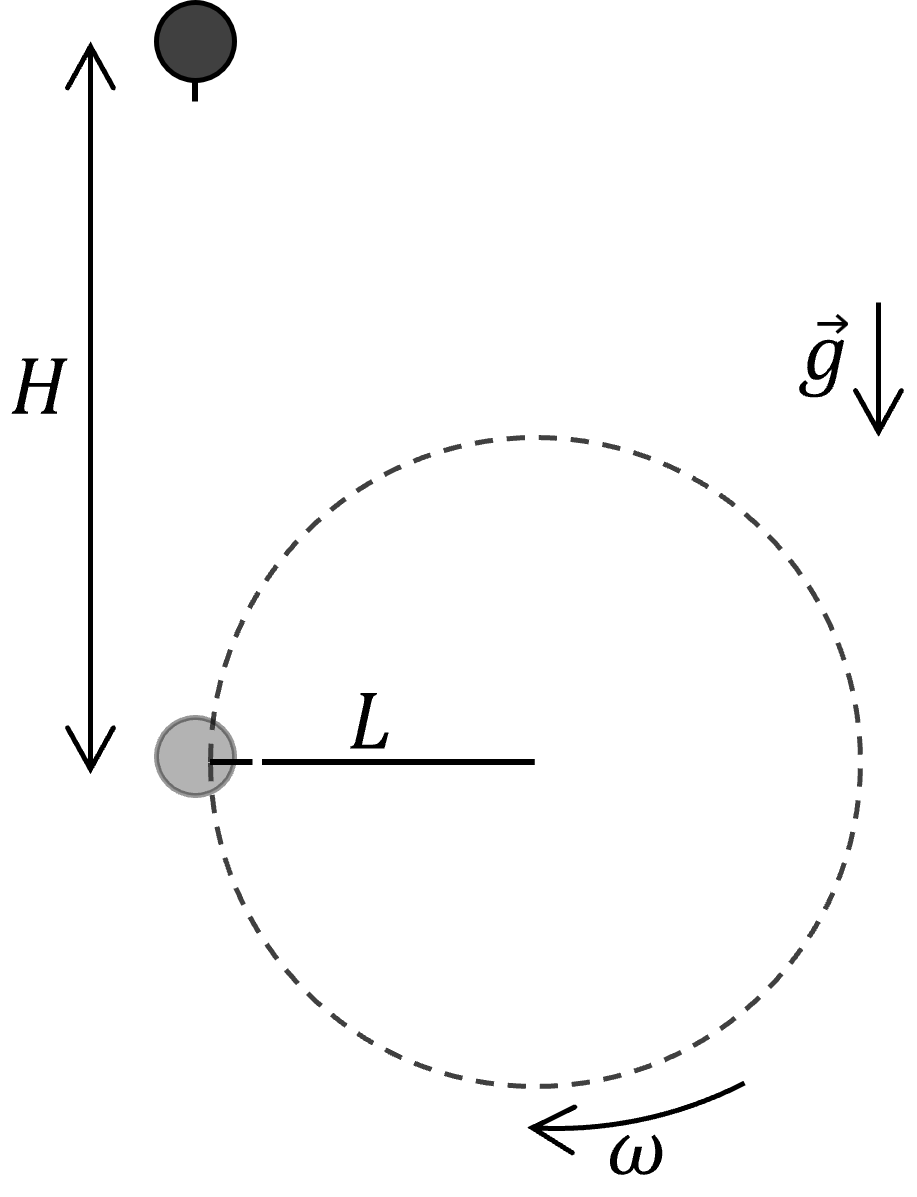
\includegraphics[width=0.2\linewidth]{2023-1/img/TD 2/piedra.png}
\end{figure}

\item Si la cuerda se hubiera cortado en un ángulo $\alpha$ con respecto a la vertical. ¿Cómo hubiera sido la trayectoria? ¿Cuál sería la velocidad inicial? Si la altura máxima alcanzada hubiera seguido siendo $H$, ¿cómo cambia su respuesta de la parte (a)?

\end{enumerate}



% Para imágenes vectoriales -> el texto tiene que estar en LaTeX
% \begin{figure}[htbp]
%   \centering
%   \svgpath{../Imagenes/ejercicios}  -> .. irse pa'trás 
%   \includesvg{ej5.svg}
% \end{figure}

\end{enumerate}
\end{document}
